\documentclass[a4paper]{article}
\renewcommand{\epsilon}{\varepsilon}
\newcommand{\triposcourse}{Methods}
\usepackage{fancyhdr,titlesec,geometry}
\usepackage[dvipsnames]{xcolor}
\usepackage[many]{tcolorbox}
\usepackage{xifthen}
\usepackage{import}
\usepackage{parskip}
\usepackage{transparent}
\usepackage{mathtools,amssymb,amsfonts,amsthm,bm}   % Math Presets
\usepackage{array,tabularx,booktabs}                % Table Presets
\usepackage{graphicx,wrapfig,float,caption}         % Figure Presets
\usepackage{setspace,multicol}                      % Text Presets
\usepackage{tikz,physics,cancel,tkz-euclide,pgfplots,tikz-3dplot}                    % Physics Presets
\usepackage{amsmath}
\usepackage{mathrsfs}
\usepackage{enumerate}
\usepackage[shortlabels]{enumitem}
\usepackage{hyperref}
\usepackage{lipsum}
\usepackage{IEEEtrantools}
\usepackage{xcomment}
\usepackage{sectsty}
\usepackage{thmtools}
\usepackage{mdframed}
\usepackage{siunitx}
\usepackage{centernot}

\newcommand{\sectionbreak}{\clearpage}

\tdplotsetmaincoords{60}{120}

\usetikzlibrary{arrows.meta}
\usetikzlibrary{decorations.markings}
\usetikzlibrary{decorations.pathmorphing}
\usetikzlibrary{automata, positioning}
\usetikzlibrary{fadings}
\usetikzlibrary{intersections}
\usetikzlibrary{cd}
\usetikzlibrary{patterns}
\usetikzlibrary{shapes.arrows}
\usepgfplotslibrary{colormaps, external}
\pgfarrowsdeclarecombine{twolatex'}{twolatex'}{latex'}{latex'}{latex'}{latex'}
\tikzset{->/.style = {decoration={markings,
                                  mark=at position 1 with {\arrow[scale=1.6]{latex'}}},
                      postaction={decorate}}}
\tikzset{<-/.style = {decoration={markings,
                                  mark=at position 0 with {\arrowreversed[scale=1.6]{latex'}}},
                      postaction={decorate}}}
\tikzset{<->/.style = {decoration={markings,
                                   mark=at position 0 with {\arrowreversed[scale=1.6]{latex'}},
                                   mark=at position 1 with {\arrow[scale=1.6]{latex'}}},
                       postaction={decorate}}}
\tikzset{->-/.style = {decoration={markings,
                                   mark=at position #1 with {\arrow[scale=1.6]{latex'}}},
                       postaction={decorate}}}
\tikzset{-<-/.style = {decoration={markings,
                                   mark=at position #1 with {\arrowreversed[scale=1.6]{latex'}}},
                       postaction={decorate}}}
\tikzset{->>/.style = {decoration={markings,
                                  mark=at position 1 with {\arrow[scale=1.6]{twolatex'}}},
                      postaction={decorate}}}
\tikzset{<<-/.style = {decoration={markings,
                                  mark=at position 0 with {\arrowreversed[scale=1.6]{twolatex'}}},
                      postaction={decorate}}}
\tikzset{<<->>/.style = {decoration={markings,
                                   mark=at position 0 with {\arrowreversed[scale=1.6]{twolatex'}},
                                   mark=at position 1 with {\arrow[scale=1.6]{twolatex'}}},
                       postaction={decorate}}}
\tikzset{->>-/.style = {decoration={markings,
                                   mark=at position #1 with {\arrow[scale=1.6]{twolatex'}}},
                       postaction={decorate}}}
\tikzset{-<<-/.style = {decoration={markings,
                                   mark=at position #1 with {\arrowreversed[scale=1.6]{twolatex'}}},
                       postaction={decorate}}}

\tikzset{
set arrow inside/.code={\pgfqkeys{/tikz/arrow inside}{#1}},
set arrow inside={end/.initial=>, opt/.initial=},
/pgf/decoration/Mark/.style={
    mark/.expanded=at position #1 with
    {
        \noexpand\arrow[\pgfkeysvalueof{/tikz/arrow inside/opt}]{\pgfkeysvalueof{/tikz/arrow inside/end}}
    }
},
arrow inside/.style 2 args={
    set arrow inside={#1},
    postaction={
        decorate,decoration={
            markings,Mark/.list={#2}
        }
    }
},
}

\tikzstyle{circ}=[fill=black, draw=black, shape=circle]
\tikzset{
dot/.style = {circle, fill, minimum size=#1,
              inner sep=0pt, outer sep=0pt},
dot/.default = 5pt% size of the circle diameter 
}
\tikzset{mstate/.style={circle, draw, blue, text=black, minimum width=0.7cm}}
\tikzset{snake it/.style={-stealth,
decoration={snake, 
    amplitude = .4mm,
    segment length = 2mm,
    post length=0.9mm},decorate}}

\def\centerarc[#1](#2)(#3:#4:#5)% Syntax: [draw options](center)(initial angle:final angle:radius)
    { \draw[#1] ($(#2)+({#5*cos(#3)},{#5*sin(#3)})$) arc (#3:#4:#5); }

\hypersetup{
    colorlinks=true,
    linkcolor=blue,
    filecolor=blue,
    citecolor = black,      
    urlcolor=cyan,
    }

%%%%%%%%%%% Snippets %%%%%%%%%%%%%%%%
\newcommand*\widefbox[1]{\fbox{\hspace{2em}#1\hspace{2em}}}
\newcommand{\xint}{\int_{x_1}^{x_2}}
\newcommand{\mw}{\sqrt{m\omega}}
\newcommand{\de}{\delta}
\newcommand{\dde}{\dot{\delta}}
\newcommand{\di}{\delta_i}
\newcommand{\ddi}{\dot{\delta_i}}
\newcommand{\dddi}{\ddot{\delta_i}}
\newcommand{\dipl}{\delta_{i+1}}
\newcommand{\dimi}{\delta_{i-1}}
\newcommand{\ddt}[1]{\frac{{d} #1}{dt}}
\newcommand{\ddtt}[1]{\frac{d^2 #1}{dt^2}}
\newcommand{\ddx}[1]{\frac{d #1}{dx}}
\newcommand{\ddxx}[1]{\frac{d^2 #1}{dx^2}}
\newcommand{\eps}{\epsilon}
\newcommand{\del}[2]{\frac{\partial #1}{\partial #2}}
\newcommand{\deltwo}[2]{\frac{\partial^2 #1}{\partial #2^2}}
\newcommand{\lam}{\lambda}
\newcommand{\Lam}{\Lambda}
\newcommand{\sig}{\sigma}
\newcommand{\Sig}{\Sigma}
\newcommand{\half}{\frac{1}{2}}
\newcommand{\munu}{{\mu\nu}}
\newcommand{\thalf}{\tfrac{1}{2}}
\renewcommand{\div}{\nabla\cdot}
\renewcommand{\curl}{\nabla\times}

\DeclareMathOperator{\orb}{Orb}
\DeclareMathOperator{\stab}{Stab}
\DeclareMathOperator{\adj}{adj}
\DeclareMathOperator{\ccl}{ccl}
\let\var\relax
\DeclareMathOperator{\var}{Var}
\DeclareMathOperator{\cov}{Cov}
\DeclareMathOperator{\corr}{Corr}
\DeclareMathOperator{\Markov}{Markov}
\DeclareMathOperator{\nullity}{nullity}

\newcommand{\bfA}{{\bf A}}
\newcommand{\bfB}{{\bf B}}
\newcommand{\bfC}{{\bf C}}
\newcommand{\bfD}{{\bf D}}
\newcommand{\bfE}{{\bf E}}
\newcommand{\bfF}{{\bf F}}
\newcommand{\bfG}{{\bf G}}
\newcommand{\bfH}{{\bf H}}
\newcommand{\bfI}{{\bf I}}
\newcommand{\bfJ}{{\bf J}}
\newcommand{\bfK}{{\bf K}}
\newcommand{\bfL}{{\bf L}}
\newcommand{\bfM}{{\bf M}}
\newcommand{\bfN}{{\bf N}}
\newcommand{\bfO}{{\bf O}}
\newcommand{\bfP}{{\bf P}}
\newcommand{\bfQ}{{\bf Q}}
\newcommand{\bfR}{{\bf R}}
\newcommand{\bfS}{{\bf S}}
\newcommand{\bfT}{{\bf T}}
\newcommand{\bfU}{{\bf U}}
\newcommand{\bfV}{{\bf V}}
\newcommand{\bfW}{{\bf W}}
\newcommand{\bfX}{{\bf X}}
\newcommand{\bfY}{{\bf Y}}
\newcommand{\bfZ}{{\bf Z}}

\newcommand{\bfa}{{\bf a}}
\newcommand{\bfb}{{\bf b}}
\newcommand{\bfc}{{\bf c}}
\newcommand{\bfd}{{\bf d}}
\newcommand{\bfe}{{\bf e}}
\newcommand{\bff}{{\bf f}}
\newcommand{\bfg}{{\bf g}}
\newcommand{\bfh}{{\bf h}}
\newcommand{\bfi}{{\bf i}}
\newcommand{\bfj}{{\bf j}}
\newcommand{\bfk}{{\bf k}}
\newcommand{\bfl}{{\bf l}}
\newcommand{\bfm}{{\bf m}}
\newcommand{\bfn}{{\bf n}}
\newcommand{\bfo}{{\bf o}}
\newcommand{\bfp}{{\bf p}}
\newcommand{\bfq}{{\bf q}}
\newcommand{\bfr}{{\bf r}}
\newcommand{\bfs}{{\bf s}}
\newcommand{\bft}{{\bf t}}
\newcommand{\bfu}{{\bf u}}
\newcommand{\bfv}{{\bf v}}
\newcommand{\bfw}{{\bf w}}
\newcommand{\bfx}{{\bf x}}
\newcommand{\bfy}{{\bf y}}
\newcommand{\bfz}{{\bf z}}

\newcommand{\mcA}{{\mathcal{A}}}
\newcommand{\mcB}{{\mathcal{B}}}
\newcommand{\mcC}{{\mathcal{C}}}
\newcommand{\mcD}{{\mathcal{D}}}
\newcommand{\mcE}{{\mathcal{E}}}
\newcommand{\mcF}{{\mathcal{F}}}
\newcommand{\mcG}{{\mathcal{G}}}
\newcommand{\mcH}{{\mathcal{H}}}
\newcommand{\mcI}{{\mathcal{I}}}
\newcommand{\mcJ}{{\mathcal{J}}}
\newcommand{\mcK}{{\mathcal{K}}}
\newcommand{\mcL}{{\mathcal{L}}}
\newcommand{\mcM}{{\mathcal{M}}}
\newcommand{\mcN}{{\mathcal{N}}}
\newcommand{\mcO}{{\mathcal{O}}}
\newcommand{\mcP}{{\mathcal{P}}}
\newcommand{\mcQ}{{\mathcal{Q}}}
\newcommand{\mcR}{{\mathcal{R}}}
\newcommand{\mcS}{{\mathcal{S}}}
\newcommand{\mcT}{{\mathcal{T}}}
\newcommand{\mcU}{{\mathcal{U}}}
\newcommand{\mcV}{{\mathcal{V}}}
\newcommand{\mcW}{{\mathcal{W}}}
\newcommand{\mcX}{{\mathcal{X}}}
\newcommand{\mcY}{{\mathcal{Y}}}
\newcommand{\mcZ}{{\mathcal{Z}}}

\newcommand{\bbA}{{\mathbb{A}}}
\newcommand{\bbB}{{\mathbb{B}}}
\newcommand{\bbC}{{\mathbb{C}}}
\newcommand{\bbD}{{\mathbb{D}}}
\newcommand{\bbE}{{\mathbb{E}}}
\newcommand{\bbF}{{\mathbb{F}}}
\newcommand{\bbG}{{\mathbb{G}}}
\newcommand{\bbH}{{\mathbb{H}}}
\newcommand{\bbI}{{\mathbb{I}}}
\newcommand{\bbJ}{{\mathbb{J}}}
\newcommand{\bbK}{{\mathbb{K}}}
\newcommand{\bbL}{{\mathbb{L}}}
\newcommand{\bbM}{{\mathbb{M}}}
\newcommand{\bbN}{{\mathbb{N}}}
\newcommand{\bbO}{{\mathbb{O}}}
\newcommand{\bbP}{{\mathbb{P}}}
\newcommand{\bbQ}{{\mathbb{Q}}}
\newcommand{\bbR}{{\mathbb{R}}}
\newcommand{\bbS}{{\mathbb{S}}}
\newcommand{\bbT}{{\mathbb{T}}}
\newcommand{\bbU}{{\mathbb{U}}}
\newcommand{\bbV}{{\mathbb{V}}}
\newcommand{\bbW}{{\mathbb{W}}}
\newcommand{\bbX}{{\mathbb{X}}}
\newcommand{\bbY}{{\mathbb{Y}}}
\newcommand{\bbZ}{{\mathbb{Z}}}

\newcommand{\mfa}{{\mathfrak{a}}}
\newcommand{\mfb}{{\mathfrak{b}}}
\newcommand{\mfc}{{\mathfrak{c}}}
\newcommand{\mfd}{{\mathfrak{d}}}
\newcommand{\mfe}{{\mathfrak{e}}}
\newcommand{\mff}{{\mathfrak{f}}}
\newcommand{\mfg}{{\mathfrak{g}}}
\newcommand{\mfh}{{\mathfrak{h}}}
\newcommand{\mfi}{{\mathfrak{i}}}
\newcommand{\mfj}{{\mathfrak{j}}}
\newcommand{\mfk}{{\mathfrak{k}}}
\newcommand{\mfl}{{\mathfrak{l}}}
\newcommand{\mfm}{{\mathfrak{m}}}
\newcommand{\mfn}{{\mathfrak{n}}}
\newcommand{\mfo}{{\mathfrak{o}}}
\newcommand{\mfp}{{\mathfrak{p}}}
\newcommand{\mfq}{{\mathfrak{q}}}
\newcommand{\mfr}{{\mathfrak{r}}}
\newcommand{\mfs}{{\mathfrak{s}}}
\newcommand{\mft}{{\mathfrak{t}}}
\newcommand{\mfu}{{\mathfrak{u}}}
\newcommand{\mfv}{{\mathfrak{v}}}
\newcommand{\mfw}{{\mathfrak{w}}}
\newcommand{\mfx}{{\mathfrak{x}}}
\newcommand{\mfy}{{\mathfrak{y}}}
\newcommand{\mfz}{{\mathfrak{z}}}

\newcommand{\mfA}{{\mathfrak{A}}}
\newcommand{\mfB}{{\mathfrak{B}}}
\newcommand{\mfC}{{\mathfrak{C}}}
\newcommand{\mfD}{{\mathfrak{D}}}
\newcommand{\mfE}{{\mathfrak{E}}}
\newcommand{\mfF}{{\mathfrak{F}}}
\newcommand{\mfG}{{\mathfrak{G}}}
\newcommand{\mfH}{{\mathfrak{H}}}
\newcommand{\mfI}{{\mathfrak{I}}}
\newcommand{\mfJ}{{\mathfrak{J}}}
\newcommand{\mfK}{{\mathfrak{K}}}
\newcommand{\mfL}{{\mathfrak{L}}}
\newcommand{\mfM}{{\mathfrak{M}}}
\newcommand{\mfN}{{\mathfrak{N}}}
\newcommand{\mfO}{{\mathfrak{O}}}
\newcommand{\mfP}{{\mathfrak{P}}}
\newcommand{\mfQ}{{\mathfrak{Q}}}
\newcommand{\mfR}{{\mathfrak{R}}}
\newcommand{\mfS}{{\mathfrak{S}}}
\newcommand{\mfT}{{\mathfrak{T}}}
\newcommand{\mfU}{{\mathfrak{U}}}
\newcommand{\mfV}{{\mathfrak{V}}}
\newcommand{\mfW}{{\mathfrak{W}}}
\newcommand{\mfX}{{\mathfrak{X}}}
\newcommand{\mfY}{{\mathfrak{Y}}}
\newcommand{\mfZ}{{\mathfrak{Z}}}

\newcommand{\rma}{\mathrm{a}}
\newcommand{\rmb}{\mathrm{b}}
\newcommand{\rmc}{\mathrm{c}}
\newcommand{\rmd}{\mathrm{d}}
\renewcommand{\dd}{\,\mathrm{d}}
\newcommand{\rme}{\mathrm{e}}
\newcommand{\rmf}{\mathrm{f}}
\newcommand{\rmg}{\mathrm{g}}
\newcommand{\rmh}{\mathrm{h}}
\newcommand{\rmi}{\mathrm{i}}
\newcommand{\rmj}{\mathrm{j}}
\newcommand{\rmk}{\mathrm{k}}
\newcommand{\rml}{\mathrm{l}}
\newcommand{\rmm}{\mathrm{m}}
\newcommand{\rmn}{\mathrm{n}}
\newcommand{\rmo}{\mathrm{o}}
\newcommand{\rmp}{\mathrm{p}}
\newcommand{\rmq}{\mathrm{q}}
\newcommand{\rmr}{\mathrm{r}}
\newcommand{\rms}{\mathrm{s}}
\newcommand{\rmt}{\mathrm{t}}
\newcommand{\rmu}{\mathrm{u}}
\newcommand{\rmv}{\mathrm{v}}
\newcommand{\rmw}{\mathrm{w}}
\newcommand{\rmx}{\mathrm{x}}
\newcommand{\rmy}{\mathrm{y}}
\newcommand{\rmz}{\mathrm{z}}
\newcommand{\rmA}{\mathrm{A}}
\newcommand{\rmB}{\mathrm{B}}
\newcommand{\rmC}{\mathrm{C}}
\newcommand{\rmD}{\mathrm{D}}
\newcommand{\rmE}{\mathrm{E}}
\newcommand{\rmF}{\mathrm{F}}
\newcommand{\rmG}{\mathrm{G}}
\newcommand{\rmH}{\mathrm{H}}
\newcommand{\rmI}{\mathrm{I}}
\newcommand{\rmJ}{\mathrm{J}}
\newcommand{\rmK}{\mathrm{K}}
\newcommand{\rmL}{\mathrm{L}}
\newcommand{\rmM}{\mathrm{M}}
\newcommand{\rmN}{\mathrm{N}}
\newcommand{\rmO}{\mathrm{O}}
\newcommand{\rmP}{\mathrm{P}}
\newcommand{\rmQ}{\mathrm{Q}}
\newcommand{\rmR}{\mathrm{R}}
\newcommand{\rmS}{\mathrm{S}}
\newcommand{\rmT}{\mathrm{T}}
\newcommand{\rmU}{\mathrm{U}}
\newcommand{\rmV}{\mathrm{V}}
\newcommand{\rmW}{\mathrm{W}}
\newcommand{\rmX}{\mathrm{X}}
\newcommand{\rmY}{\mathrm{Y}}
\newcommand{\rmZ}{\mathrm{Z}}

\newcommand{\GL}{\mathrm{GL}}
\newcommand{\Or}{\mathrm{O}}
\newcommand{\PGL}{\mathrm{PGL}}
\newcommand{\PSL}{\mathrm{PSL}}
\newcommand{\PSO}{\mathrm{PSO}}
\newcommand{\PSU}{\mathrm{PSU}}
\newcommand{\SL}{\mathrm{SL}}
\newcommand{\SO}{\mathrm{SO}}
\newcommand{\Spin}{\mathrm{Spin}}
\newcommand{\Sp}{\mathrm{Sp}}
\newcommand{\SU}{\mathrm{SU}}
\newcommand{\Mat}{\mathrm{Mat}}

% Some common notations

\renewcommand{\v}{\mathbf{v}}
\newcommand{\w}{\mathbf{w}}
\renewcommand{\u}{\mathbf{u}}

% Matrix algebras
\newcommand{\gl}{\mathfrak{gl}}
\newcommand{\ort}{\mathfrak{o}}
\newcommand{\so}{\mathfrak{so}}
\newcommand{\su}{\mathfrak{su}}
\newcommand{\uu}{\mathfrak{u}}
\renewcommand{\sl}{\mathfrak{sl}}
\newcommand{\inner}[1]{\left\langle{#1}\right\rangle}
\DeclareMathOperator{\spn}{span}

\newcommand{\mobius}{{M\"{o}bius }}

\renewcommand{\ge}{\geqslant}
\renewcommand{\le}{\leqslant}
\renewcommand{\geq}{\geqslant}
\renewcommand{\leq}{\leqslant}
\renewcommand{\restriction}{\mathord{\upharpoonright}}

\newcommand\independent{\protect\mathpalette{\protect\independenT}{\perp}}
\def\independenT#1#2{\mathrel{\rlap{$#1#2$}\mkern2mu{#1#2}}}

\setlength{\parindent}{0pt}
% \setlength{\parskip}{\baselineskip}
\newcommand{\incfig}[1]{%
    \def\svgwidth{0.4\columnwidth}
    \import{./figures/}{#1.pdf_tex}
}
%%%%%%%%%%%%%%%%%%%%%%%%%%%%%%%%%%%%%

\usepackage[T1]{fontenc}
\usepackage{lmodern,mathrsfs}

%%%%%%%boxed enviroment for final layout%%%%%%%%%%%%%

\newtheoremstyle{mystyle}%
  {}%
  {}%
  {}%
  {}%
  {\sffamily\bfseries}%
  {.}%
  { }%
  {}%

% \renewenvironment{proof}{{\sffamily\bfseries Proof. }}{\qed}

\theoremstyle{mystyle}{
  \newtheorem{theorem}{Theorem}[section]
  \newtheorem{lemma}[theorem]{Lemma}
  \newtheorem{proposition}[theorem]{Proposition}
  \newtheorem{corollary}[theorem]{Corollary}
  \newtheorem{problem}[theorem]{Problem}
  \newtheorem*{claim}{Claim}
  \newtheorem*{slemma}{Lemma}
  \newtheorem*{sprop}{Proposition}
  \newtheorem*{notation}{Notation}

  \newtheorem{inquestion}{Question}
  \newtheorem*{sque}{Question}

  \newtheorem{definition}{Definition}[section]
  \newtheorem{conjecture}{Conjecture}[section]
  \newtheorem{example}{Example}[section]
  \newtheorem*{law}{Law}

  \newtheorem*{remark}{Remark}
  \newtheorem*{note}{Note}
}

\newenvironment{question}[1]
{\renewcommand\theinquestion{#1}\inquestion}
{\endinquestion}

\theoremstyle{definition}{
    \newtheorem*{exercise}{Exercise}}

\tcolorboxenvironment{definition}{
  boxrule=0pt,
  boxsep=2pt,
  colback={White!90!Cerulean},
  enhanced jigsaw, 
  borderline west={2pt}{0pt}{Cerulean},
  sharp corners,
  before skip=10pt,
  after skip=10pt,
  breakable,
  % parbox=false,
}

\tcolorboxenvironment{notation}{
  boxrule=0pt,
  boxsep=2pt,
  colback={White!90!Cerulean},
  enhanced jigsaw, 
  borderline west={2pt}{0pt}{Cerulean},
  sharp corners,
  before skip=10pt,
  after skip=10pt,
  breakable,
  % parbox=false,
}

\tcolorboxenvironment{proposition}{
  boxrule=0pt,
  boxsep=2pt,
  colback={White!90!Yellow},
  enhanced jigsaw, 
  borderline west={2pt}{0pt}{Yellow},
  sharp corners,
  before skip=10pt,
  after skip=10pt,
  breakable,
  % parbox=false,
}

\tcolorboxenvironment{sprop}{
  boxrule=0pt,
  boxsep=2pt,
  colback={White!90!Yellow},
  enhanced jigsaw, 
  borderline west={2pt}{0pt}{Yellow},
  sharp corners,
  before skip=10pt,
  after skip=10pt,
  breakable,
  % parbox=false,
}

\tcolorboxenvironment{theorem}{
  boxrule=0pt,
  boxsep=2pt,
  colback={White!90!Dandelion},
  enhanced jigsaw, 
  borderline west={2pt}{0pt}{Dandelion},
  sharp corners,
  before skip=10pt,
  after skip=10pt,
  breakable,
  % parbox=false,
}

\tcolorboxenvironment{lemma}{
  boxrule=0pt,
  boxsep=2pt,
  blanker,
  borderline west={2pt}{0pt}{Red},
  before skip=10pt,
  after skip=10pt,
  sharp corners,
  left=12pt,
  right=12pt,
  breakable,
  % parbox=false,
}

\tcolorboxenvironment{corollary}{
  boxrule=0pt,
  boxsep=2pt,
  blanker,
  borderline west={2pt}{0pt}{ForestGreen},
  before skip=10pt,
  after skip=10pt,
  sharp corners,
  left=12pt,
  right=12pt,
  breakable,
  % parbox=false,
}

\tcolorboxenvironment{proof}{
  boxrule=0pt,
  boxsep=2pt,
  blanker,
  borderline west={2pt}{0pt}{NavyBlue!80!white},
  before skip=10pt,
  after skip=10pt,
  left=12pt,
  right=12pt,
  breakable,
  % parbox=false,
}

\tcolorboxenvironment{remark}{
  boxrule=0pt,
  boxsep=2pt,
  blanker,
  borderline west={2pt}{0pt}{Green},
  before skip=10pt,
  after skip=10pt,
  left=12pt,
  right=12pt,
  breakable,
  % parbox=false,
}

\tcolorboxenvironment{note}{
  boxrule=0pt,
  boxsep=2pt,
  blanker,
  borderline west={2pt}{0pt}{PineGreen},
  before skip=10pt,
  after skip=10pt,
  left=12pt,
  right=12pt,
  breakable,
  % parbox=false,
}

\tcolorboxenvironment{example}{
  boxrule=0pt,
  boxsep=2pt,
  blanker,
  borderline west={2pt}{0pt}{Black},
  sharp corners,
  before skip=10pt,
  after skip=10pt,
  left=12pt,
  right=12pt,
  breakable,
  % parbox=false,
}

\titleformat*{\section}{\Large\bfseries\sffamily}
\titleformat*{\subsection}{\large\bfseries\sffamily}
\titleformat*{\subsubsection}{\bfseries\sffamily}
\titleformat*{\paragraph}{\bfseries\sffamily}

%%%%%%%%%%%%%%%%%%%%%%%%%%%%%%%%%%%%%%%%%%%%%%%%%%%%

\title{\textbf{\sffamily\triposcourse{} Notes}}
% \usepackage[T1]{fontenc}
\usepackage{crimson}

\theoremstyle{plain}

\theoremstyle{definition}
\newtheorem{theorem}{Theorem}[section]
\newtheorem{lemma}[theorem]{Lemma}
\newtheorem{proposition}[theorem]{Proposition}
\newtheorem{corollary}[theorem]{Corollary}
\newtheorem{problem}[theorem]{Problem}
\newtheorem*{claim}{Claim}
\newtheorem*{slemma}{Lemma}
\newtheorem*{sprop}{Proposition}
\newtheorem*{notation}{Notation}
\newtheorem*{exercise}{Exercise}

\newtheorem{inquestion}{Question}
\newtheorem*{sque}{Question}
\newenvironment{question}[1]
  {\renewcommand\theinquestion{#1}\inquestion}
  {\endinquestion}

\newtheorem{definition}{Definition}[section]
\newtheorem{conjecture}{Conjecture}[section]
\newtheorem{example}{Example}[section]
\newtheorem*{law}{Law}

\theoremstyle{remark}
\newtheorem*{remark}{Remark}
\newtheorem*{note}{Note}

\title{\textbf{\triposcourse{} Notes}}
% \theoremstyle{plain}{
  \newtheorem{theorem}{Theorem}[section]
  \newtheorem{lemma}[theorem]{Lemma}
  \newtheorem{proposition}[theorem]{Proposition}
  \newtheorem{corollary}[theorem]{Corollary}
  \newtheorem*{claim}{Claim}
  \newtheorem*{slemma}{Lemma}
  \newtheorem*{sprop}{Proposition}
  \newtheorem{conjecture}{Conjecture}[section]
  \newtheorem*{law}{Law}
  \newtheorem{inquestion}{Question}
  \newtheorem*{sque}{Question}
}

\theoremstyle{definition}{
  \newtheorem{method}[theorem]{Method}
  \newtheorem{definition}{Definition}[section]
  \newtheorem{example}{Example}[section]
  \newtheorem*{notation}{Notation}
  \newtheorem*{exercise}{Exercise}
}

\theoremstyle{remark}{
  \newtheorem{remark}[theorem]{Remark}
  \newtheorem*{note}{Note}
}

\newenvironment{question}[1]
{\renewcommand\theinquestion{#1}\inquestion}
{\endinquestion}

\title{\textbf{\sffamily\triposcourse{} Notes}}

%layout full
% \geometry{%
%   a4paper,
%   lmargin=2cm,
%   rmargin=2.5cm,
%   tmargin=3.5cm,
%   bmargin=2.5cm,
%   footskip=12pt,
%   headheight=24pt}
% layout trim
% \geometry{
% papersize={379pt, 542pt},
% textwidth=345pt,
% textheight=443pt,
% left=17pt,
% top=54pt,
% right=17pt
% }
% layout a5
\geometry{%
  a5paper,
  lmargin=1cm,
  rmargin=1cm,
  tmargin=2.5cm,
  bmargin=1.5cm,
  footskip=15pt,
  headheight=24pt}
\pagestyle{fancy}
\rhead{{\triposcourse{}}}
\author{jt775}
\AddToHook{cmd/section/before}{\clearpage}

\graphicspath{ {./images/} }
\pgfplotsset{compat=1.17}
\begin{document}
\maketitle
\tableofcontents
\newpage
\part*{Lecture 1}
\part{Self-adjoint ODEs}
\section{Fourier Series}
\subsection{Periodic functions}
\begin{definition}
    A function $f$ is \textit{periodic} if $ f(x+T)=f(x), \forall x $, where $T$ is the period.
\end{definition}
\begin{center}
    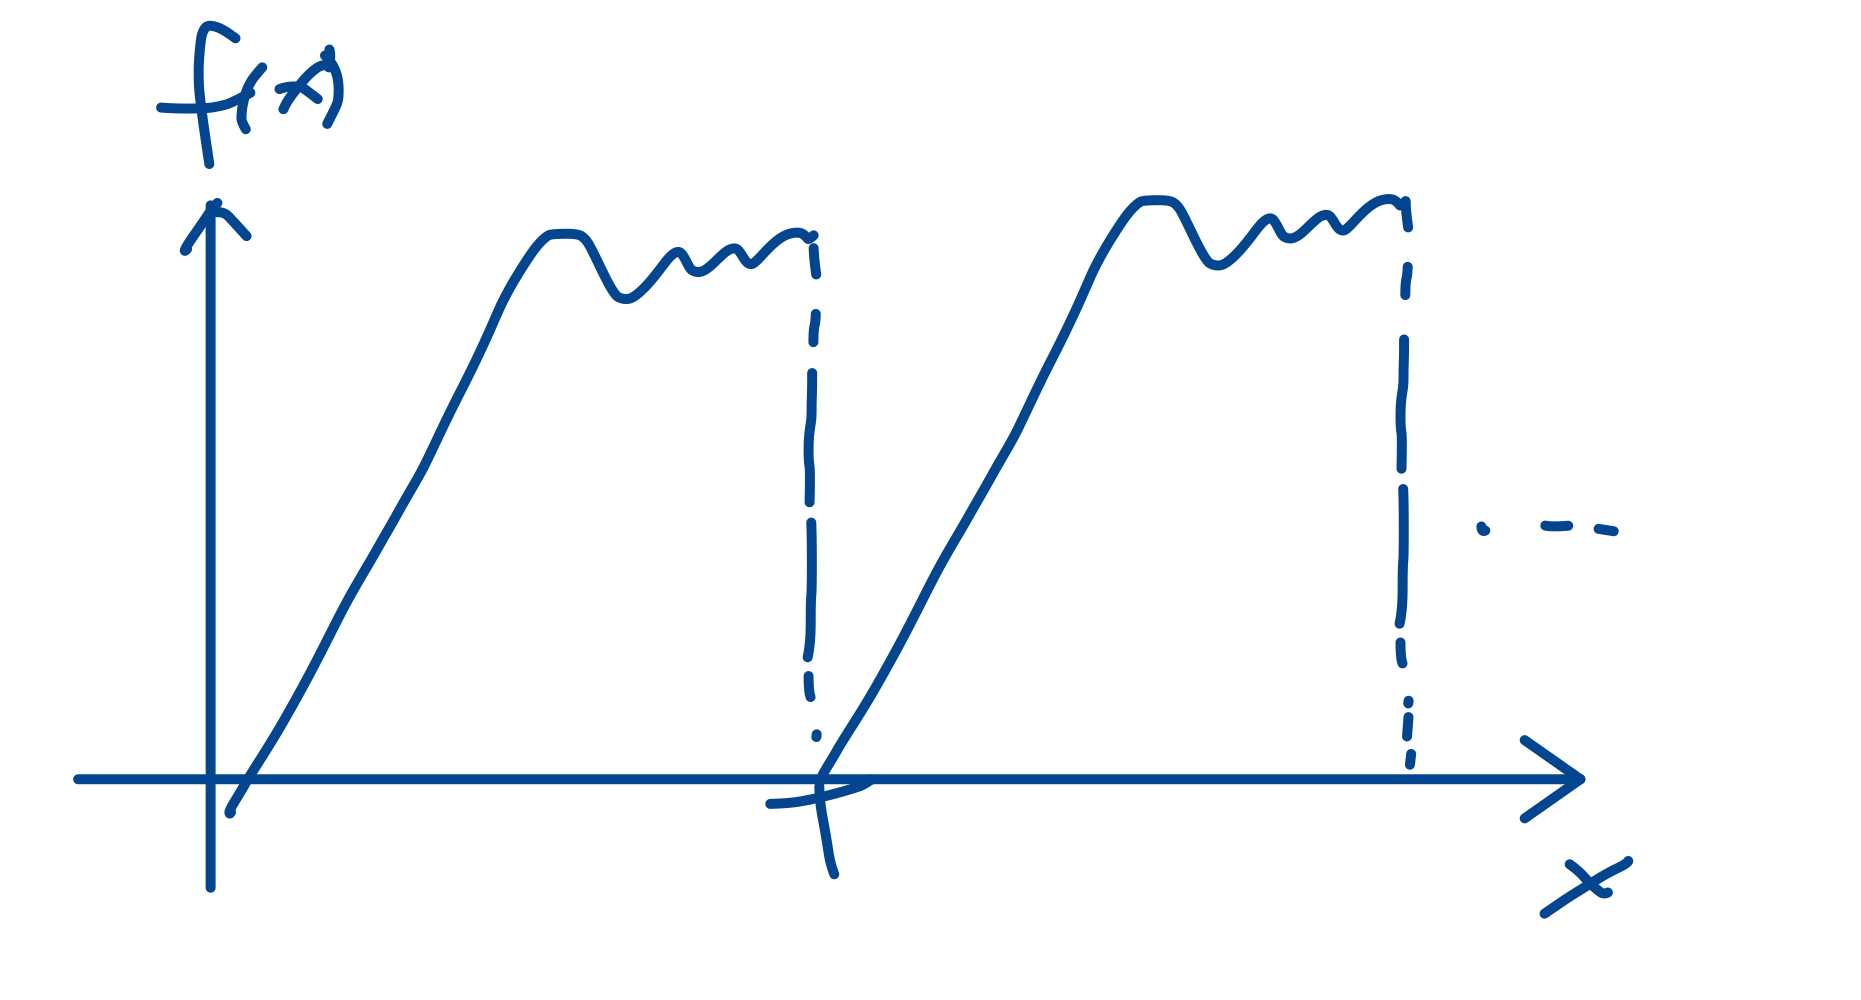
\includegraphics[scale=0.1]{methods1.jpeg}
\end{center}
Consider the set of functions 
\[
    g_n(x) = \cos \left( \frac{n\pi x}{L} \right),\quad h_n(x) = \sin \left( \frac{n\pi x}{L} \right).
\]
They are periodic on $ [0,2L] $ with period 2L.

Recall identities
\[
    \begin{aligned} \cos (A \pm B) &=\cos A \cos B \mp \sin A \sin B \\ \sin (A \pm B) &=\sin A \cos B \pm \cos A \sin B, \text { and so } \\ \cos A \cos B &=\frac{1}{2}[\cos (A-B)+\cos (A+B)] \\ \sin A \sin B &=\frac{1}{2}[\cos (A-B)-\cos (A+B)] \\ \sin A \cos B &=\frac{1}{2}[\sin (A+B)+\sin (A-B)] \end{aligned}
\]
Define an inner product of the set 
\[
    \langle f,g \rangle = \int_{0}^{2L} f(x)g(x)\,\mathrm{d}x.
\]
\begin{proposition}
    With this inner product, $g_n,h_n$ are mutually orthogonal on $ [0,2L) $.
\end{proposition}
\begin{proof}
    Check that
    \[
        \langle h_n,h_m \rangle = \begin{cases}
            L\delta_{nm} &\forall n,m\neq 0\\
            0 & m=0 \lor n=0\\
            \end{cases} \quad
            \langle g_n,g_m \rangle = \begin{cases}
            L \delta_{mn} &n,m\neq 0\\
            2L \delta_{0n} & m=0\\
            \end{cases} \quad
            \langle h_n,g_m \rangle =0.
    \]
\end{proof}
$g_n,h_n$ form a complete orthogonal set, i.e. they span the space of well-behaved periodic functions $ [0,2L) $ and they are linearly independent.

\subsection{Definition of Fourier series}
We can express any well-behaved periodic function of period 2L as 
\[
    f(x) = \frac{1}{2}a_0 + \sum_{n=1}^{\infty} a_n \cos \left( \frac{n\pi x}{L} \right)+ \sum_{n=1}^{\infty} b_n \sin \left( \frac{n\pi x}{L} \right)\tag{$*$}
\]
where $a_n,b_n$ are constants such that RHS is convergent for all $x$ where $f$ is continuous. At a discontinuity $x$, the Fourier series approaches the midpoint of upper and lower limits at $x$, i.e. 
\[
    \frac{f(x_+)+f(x_-)}{2} = \frac{1}{2}a_0 + \sum_{n=1}^{\infty} a_n \cos \left( \frac{n\pi x}{L} \right)+ \sum_{n=1}^{\infty} b_n \sin \left( \frac{n\pi x}{L} \right).
\]
Consider $ \langle h_n,f \rangle  $ and substitute in ($ * $), we get 
\[
    \int_{0}^{2L} \sin \left( \frac{n \pi x}{L} \right) f(x) \,\mathrm{d}x = \sum_{m=1}^{\infty}Lb_m \delta_{nm} = Lb_n.
\]
Similar for $a_n$. We get
\[
    b_{n}=\frac{1}{L} \int_{0}^{2 L} f(x) \sin \left(\frac{n \pi x}{L}\right)\, \rmd x,\quad a_n = \frac{1}{L}\int_{0}^{2L} f(x) \cos \left( \frac{n \pi x}{L} \right) \,\mathrm{d}x.
\]
\begin{note}
    \begin{enumerate}
        \item $a_n$ includes $n=0$ since $ \frac{1}{2}a_0 $ is the average of $f$, i.e.
        \[
            \langle f \rangle = \frac{1}{2L}\int_{0}^{2L} f(x) \,\mathrm{d}x.
        \]
        \item Range of integration can be changed as long as it has length $2L$. We usually consider $ \int_{-L}^{L} $.
        \item Can think of the Fourier series as the decomposition into harmonics. The simplest Fourier series are sines and cosines. e.g. $ \sin (3 \pi x/ L) $ has Fourier series $b_3=1$ and $ b_n=0,n\neq 3 ,a_n=0$.
    \end{enumerate}
\end{note}
\begin{example}[Sawtooth wave]
    Consider $f(x)=x,x\in [-L,L)$ and periodic elsewhere.
    \begin{center}
        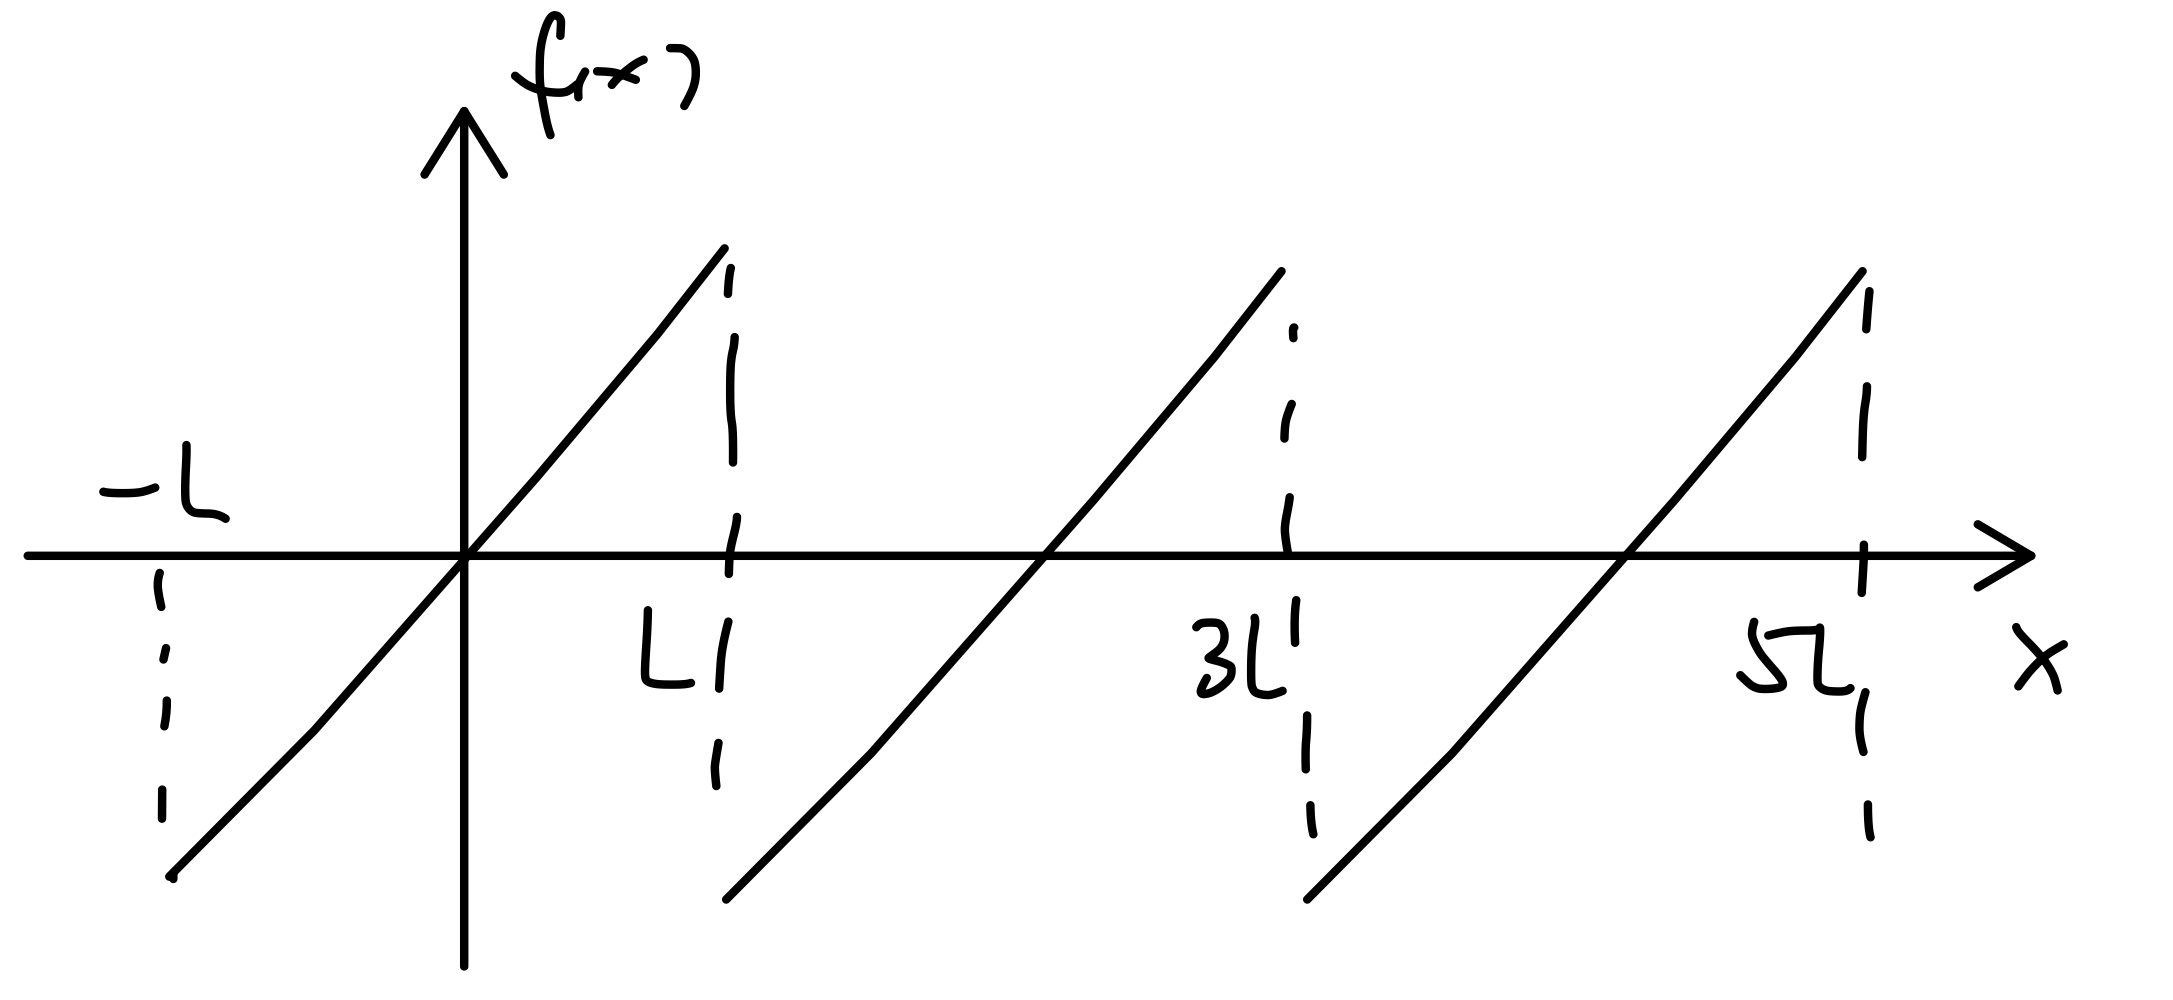
\includegraphics[scale=0.1]{methods2.jpeg}
    \end{center}
    We have 
    \begin{align*}
        a_n &= \frac{1}{L}\int_{-L}^{L} x\cdot \cos \left( \frac{n\pi x}{L} \right) \,\mathrm{d}x=0,\\ 
        b_n &= \frac{2}{L} \int_{0}^{L} x\cdot \sin \left( \frac{n\pi x}{L} \right) \,\mathrm{d}x = \frac{2L}{n\pi }(-1)^{n+1}.
    \end{align*}
    So the Fourier series is 
    \[
        f(x) = \frac{2L}{\pi } \sum_{n=1}^{\infty}\frac{(-1)^{n+1}}{n}\sin \left( \frac{n\pi x}{L} \right).
    \]
\end{example}
\begin{note}
    As $n\to \infty$ in Fourier series,
    \begin{enumerate}
        \item The FS approximation improves (convergent where continuous).
        \item FS $ \to 0 $ at $x=L$, i.e. the midpoint of continuity.
        \item FS has a persistent \textit{overshoot} at $x=L$, which is approximately 9\% and is known as the \textit{Gibbs phenonenon}. See Example Sheet Q5.
    \end{enumerate}
\end{note}
\newpage
\part*{Lecture 2}
\subsection{The Dirichlet Conditions and Fourier's Theorem}
A natural question is then which functions are allowed to have a proper Fourier series.
Surprisingly, a big, yet hard to precisely characterise, class of functions has a convergent Fourier series that has the desired properties.
This class even includes some classical counterexamples in analysis.
As an applied course, we will just look at some of the sufficient conditions.
\begin{theorem}[Fourier's Theorem]
    If $f$ is a bounded periodic function with period $2L$ with a finite number of minima, maxima, and discontinuities in $[0,2L)$, then its Fourier series converges to $f$ where it is continuous and converges to the average of the two side limits.
\end{theorem}
The conditions in this theorem is known as the Dirichlet conditions.
\begin{note}
    \begin{enumerate}
        \item These conditions are hella weak compared to our conditions for a function to have e.g. a Taylor series.
        However, pathological functions like $1/x,\sin(1/x),1_{\mathbb R\setminus\mathbb Q}(x)$ are excluded from these conditions.
        \item The converse is not true, as $\sin(1/x)$ has a Fourier series we desire.
    \end{enumerate}
\end{note}
\begin{proof}
    See Jeffery \& Jeffery book.
\end{proof}
Another subject of interest is the rate of convergence of a Fourier series.
Perhaps unsurprisingly, it depends on the smoothness of the function.
\begin{theorem}
    If $f(x)$ is $p^{th}$ differentiable but $f^{(p)}$ is not continuous, then its Fourier series converges as $O(n^{-(p+1)})$ as $n\to\infty$.
\end{theorem}
\begin{example}
    \begin{enumerate}
        \item  Consider the square wave
        $$f(x)=\begin{cases}
            1\text{, for $0\le x<1$}\\
            -1\text{, for $-1\le x<0$}
        \end{cases}$$
        That extends periodically with period $2$.
        Then it has a Fourier series
        $$4\sum_{m=1}^\infty\frac{\sin[(2m-1)\pi x]}{(2m-1)\pi}$$
        which, as one can see both from the preceding theorem (with $p=0$) and observation, converges slowly.
        \item Consider the general ``see-saw'' wave
        $$f(x)=\begin{cases}
            x(1-\xi)\text{, for $x\in[0,\xi)$}\\
            \xi(1-x)\text{, for $x\in[\xi,1)$}
        \end{cases}$$
        which extends as an odd periodic function with period $2$.
        This has Fourier series
        $$2\sum_{m=1}^\infty\frac{\sin (n\pi\xi)\sin (n\pi x)}{(n\pi)^2}$$
        which converges with $p=1$ in the preceding theorem.
        In particular, $\xi=1/2$ gives
        $$2\sum_{m=1}^\infty(-1)^{m+1}\frac{\sin[(2m-1)\pi x]}{[(2m-1)\pi]^2}$$
        which can be seen, immediately, that it converges faster than the series in the previous example.
        \item Take $f(x)=x(1-x)/2$ for $x\in[0,1)$ that extends as an odd periodic function with period $2$.
        Then its Fourier series is
        $$4\sum_{m=1}^\infty\frac{\sin[(2m-1)\pi x]}{[(2m-1)\pi]^3}$$
        which has $p=2$.
        \item Take $f(x)=(1-x^2)^2$, then $a_n=O(n^{-4})$.
    \end{enumerate}
\end{example}
Of course, we want to integrate and differentiate a Fourier series term-by-term.
Integration, as one expect, seldom yields problems as it imposed very few restrictions on the function.

And indeed, we are just going to assume we can integrate any Fourier series term-by-term and they guarantee to yield a smoother function, which satisfies the Dirichlet conditions if the original function does.

Differentiation is more problematic when doing it term-by-term.
\begin{example}
    Take the square wave again which is known to have Fourier series
    $$4\sum_{m=1}^\infty\frac{\sin[(2m-1)\pi x]}{(2m-1)\pi}$$
    which, after term-by-term differentiation, yields
    $$4\sum_{m=1}^\infty\cos[(2m-1)\pi x]$$
    which is clearly divergent.
    This is perhaps unsurprising as the original function is not even continuous.
\end{example}
\begin{theorem}
    If $f(x)$ is differentiable and both $f,f^\prime$ satisfy Dirichlet conditions, then we can differentiate the Fourier series of $f$ term-by-term to get the Fourier series of $f^\prime$.
\end{theorem}
\begin{example}
    If we differentiate the see-saw curve with $\xi=1/2$, then we will get an offset of the Fourier series of the square wave with $ \tilde{x}=x+1/2 $.
\end{example}
\subsection{Parseval's Theorem}
There is some interesting relation between the integral of the square of a function and the square of the Fourier coefficients of that function.
If the function is nice enough to have a nice enough Fourier series, then by orthogonality,
\begin{align*}
    \int_0^{2L}f(x)^2\,\mathrm dx&=\int_0^{2L}\left( \frac{a_0}{2}+\sum_{n\ge 1}a_n\cos\frac{n\pi x}{L}+\sum_{n\ge 1}b_n\sin\frac{n\pi x}{L} \right)^2\,\mathrm dx\\
    &=\int_0^{2L}\left( \frac{a_0^2}{4}+\sum_{n\ge 1}a_n^2\cos^2\frac{n\pi x}{L}+\sum_{n\ge 1}b_n^2\sin^2\frac{n\pi x}{L} \right)\,\mathrm dx\\
    &=L\left( \frac{a_0^2}{2}+\sum_{n\ge 1}(a_n^2+b_n^2) \right).
\end{align*}
This is also called the \textit{completeness relation} as the left hand side would be greater than or equal to the right hand side if any basis functions are missing from the series.
This is known as Parseval's Theorem.
\begin{theorem}[Parseval's Theorem]\label{parseval}
    For a nice enough function $f$ with Fourier coefficients $a_n,b_n$, we have
    $$\int_0^{2L}f(x)^2\,\mathrm dx=L\left( \frac{a_0^2}{2}+\sum_{n\ge 1}(a_n^2+b_n^2) \right)$$
\end{theorem}
\begin{proof}
    Above.
\end{proof}
\begin{example}
    Consider the sawtooth curve with $f(x)=x,x\in[-L,L)$ with period $2L$.
    Then Parseval's Theorem reveals that
    $$\frac{2}{3}L^3=\int_{-L}^Lx^2\,\mathrm dx=L\sum_{n=1}^\infty\frac{4L^2}{n^2\pi^2}=\frac{4L^3}{\pi^2}\sum_{n=1}^\infty\frac{1}{n^2}\implies \sum_{n=1}^\infty\frac{1}{n^2}=\frac{\pi^2}{6}$$
\end{example}
\begin{remark}
    If we think of the integral of the square as $ \langle f,f \rangle = \left\| f \right\| ^2  $, the $ L^2 $ norm, then Parseval's Theorem can be thought of an analog of Pythagoras' Theorem in this space of functions.
\end{remark}
\newpage
\part*{Lecture 3}
\end{document}